\section{tasks::subtract\-Frames Class Reference}
\label{classtasks_1_1subtractFrames}\index{tasks::subtractFrames@{tasks::subtractFrames}}
Inheritance diagram for tasks::subtract\-Frames::\begin{figure}[H]
\begin{center}
\leavevmode
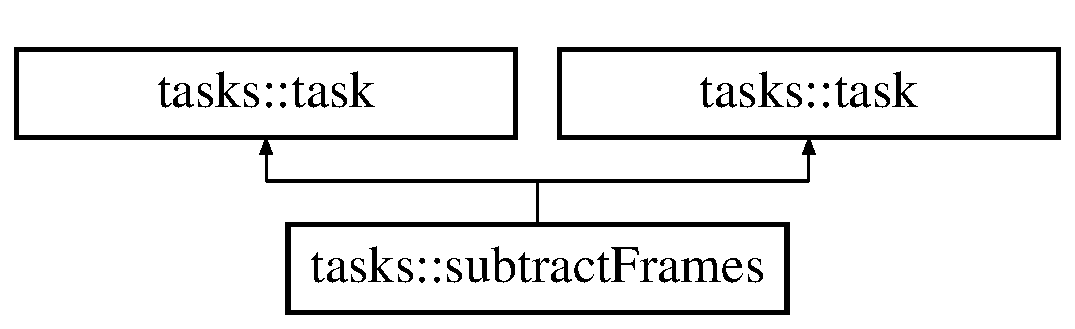
\includegraphics[height=2cm]{classtasks_1_1subtractFrames}
\end{center}
\end{figure}
\subsection*{Public Member Functions}
\begin{CompactItemize}
\item 
def \textbf{\_\-\_\-init\_\-\_\-}\label{classtasks_1_1subtractFrames_9925214ff2d01c57ef271246f9328c55}

\item 
def \textbf{run}\label{classtasks_1_1subtractFrames_e072c754659b6971f4dd98a90d9170e1}

\item 
def \textbf{\_\-\_\-init\_\-\_\-}\label{classtasks_1_1subtractFrames_9925214ff2d01c57ef271246f9328c55}

\item 
def \textbf{run}\label{classtasks_1_1subtractFrames_e072c754659b6971f4dd98a90d9170e1}

\end{CompactItemize}
\subsection*{Static Public Attributes}
\begin{CompactItemize}
\item 
string \textbf{name} = '{\bfsubtract\-Frames}'\label{classtasks_1_1subtractFrames_2618b923070421fdf3a02526aa2b22b6}

\item 
string \textbf{button\-Text} = '{\bfsubtract\-Frames}'\label{classtasks_1_1subtractFrames_ae4b8667f92f9c37fa53b770f63b2f10}

\item 
int \textbf{inthread} = 0\label{classtasks_1_1subtractFrames_df4128c3c177cd613be440948928fe23}

\end{CompactItemize}


\subsection{Detailed Description}


\footnotesize\begin{verbatim}Subtract two selected frames
\end{verbatim}
\normalsize
 



The documentation for this class was generated from the following files:\begin{CompactItemize}
\item 
old/PANICtool-1.0/tasks.py\item 
old/tasks.py\end{CompactItemize}
